\textnormal{
The programming language we use for this project is Python 2.7, the programming environment is Windows 64-bit.
%Building the corresponding relational tables, according to the proposed ER model described in the previous phase %enforcing the different integrity constraints.  
The deliverables for this stage include the following items:
\begin{itemize} 
\item{Data Snippet: See Fig.2}
\begin{figure}
\centering
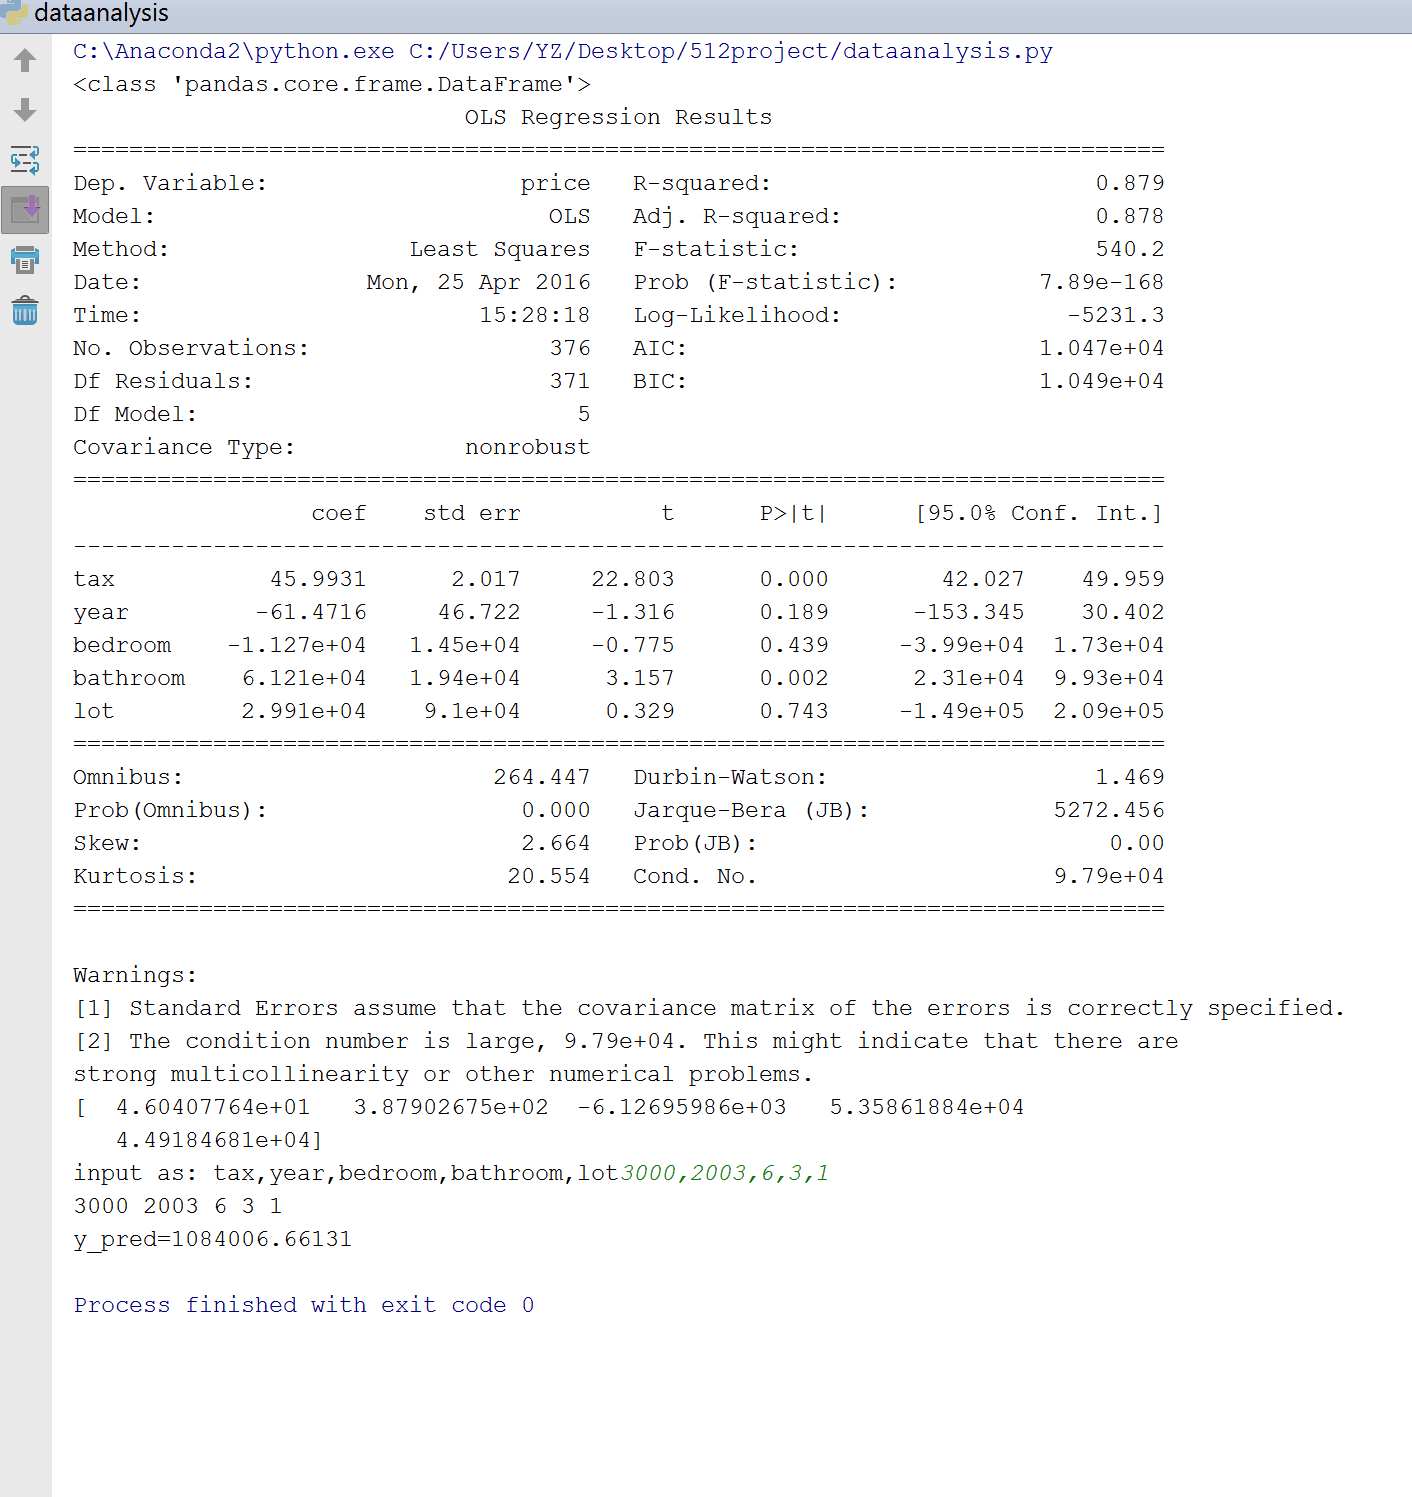
\includegraphics[width=0.5\textwidth]{RegressionPredictionOutput.png}
\caption{}
\end{figure}
%The SQL tables that represent the ER project model, along with at least 3-5 rows of concrete data per table.
\item{Regression and Prediction: See Fig.3}
\begin{figure}
\centering
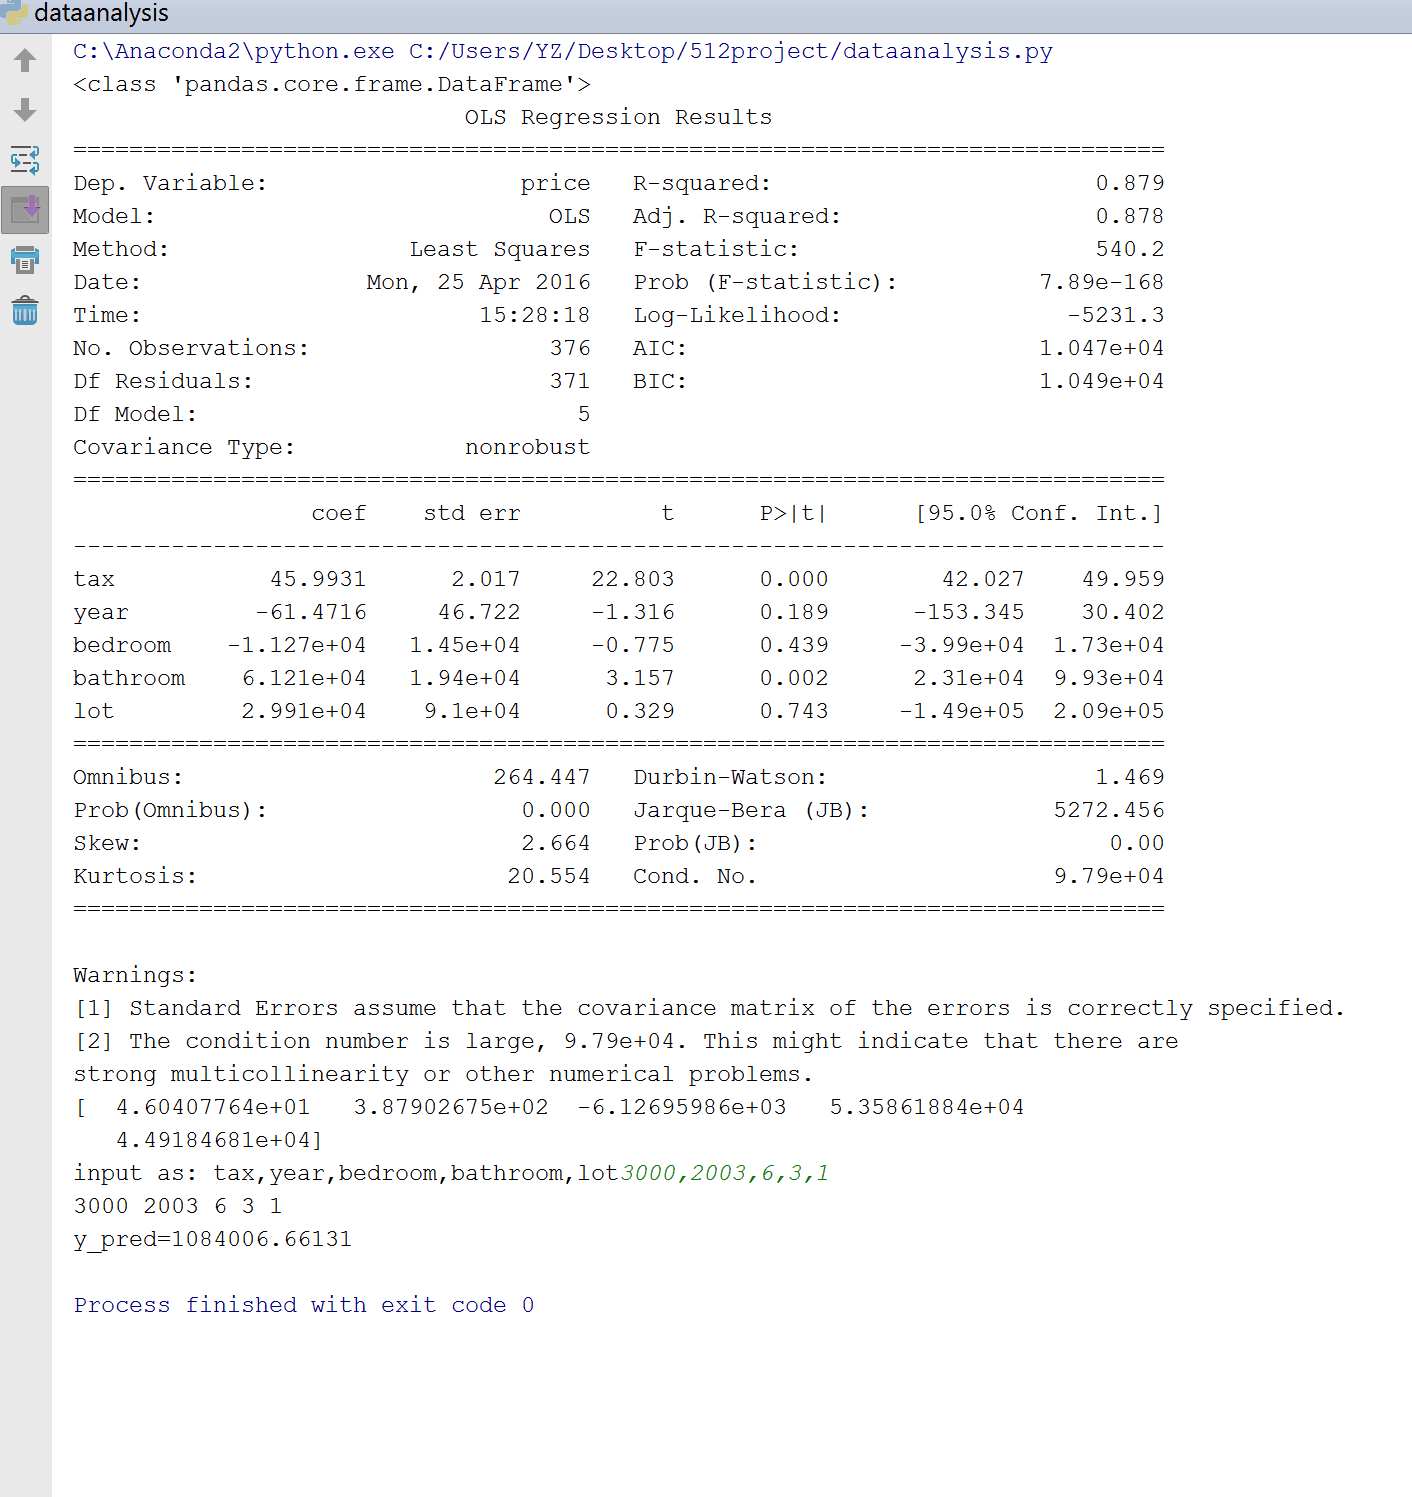
\includegraphics[width=0.5\textwidth]{RegressionPredictionOutput.png}
\caption{}
\end{figure}
%The normalization steps for each table, along with explanations/justifications of each normalization step.
\item{Datacrawling: See Fig.4-6}
\begin{figure}
\centering
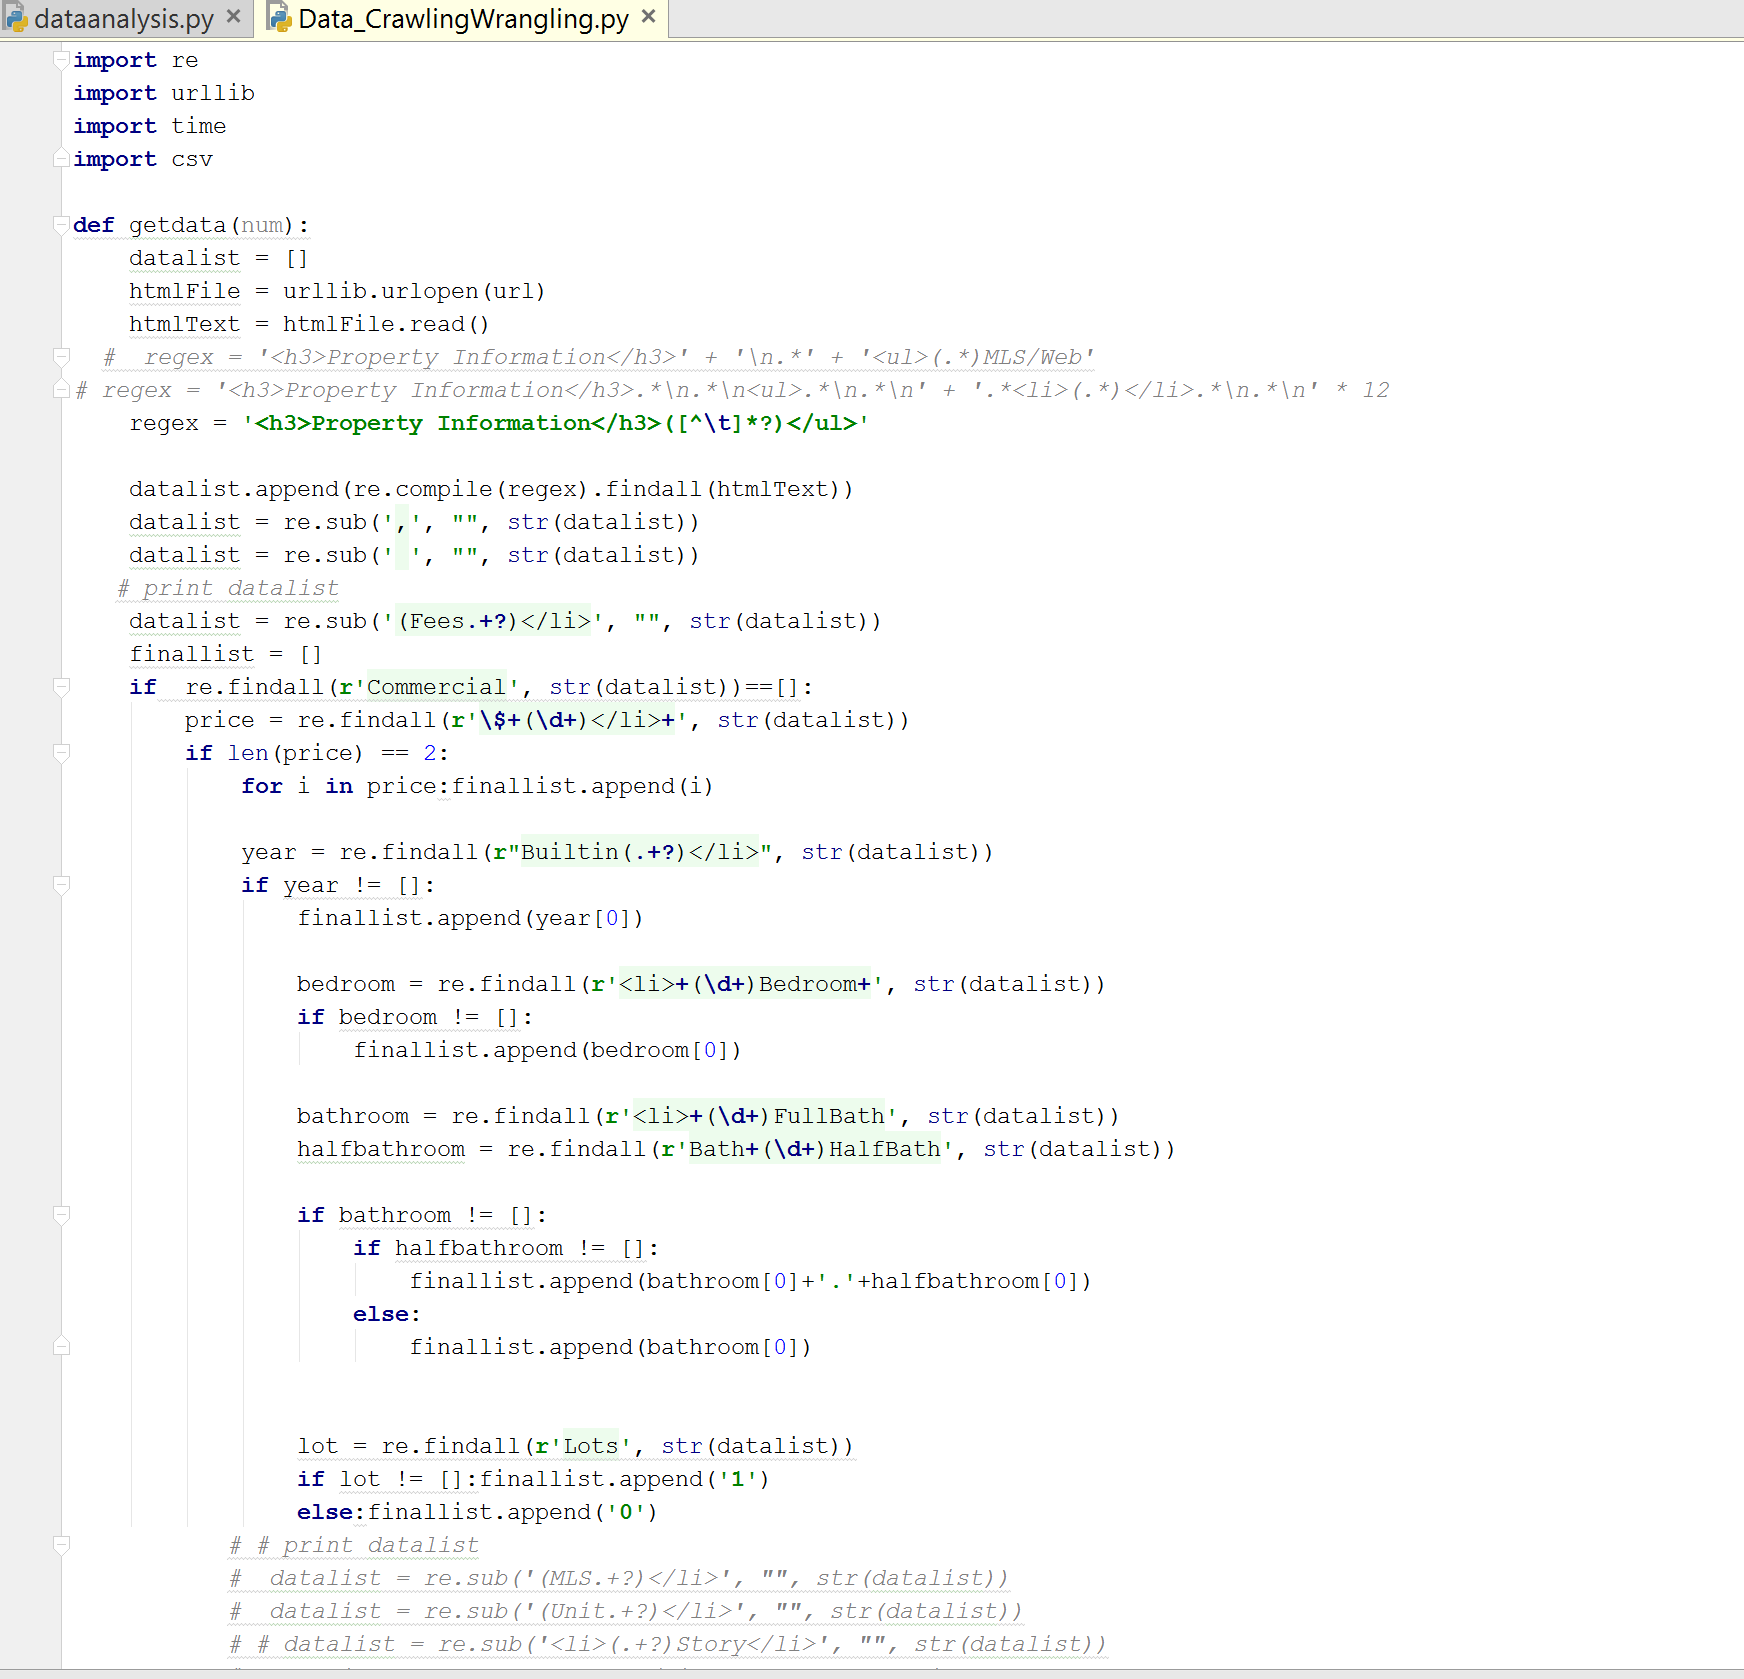
\includegraphics[width=0.5\textwidth]{datacrawling1.png}
\caption{}
\end{figure}
\begin{figure}
\centering
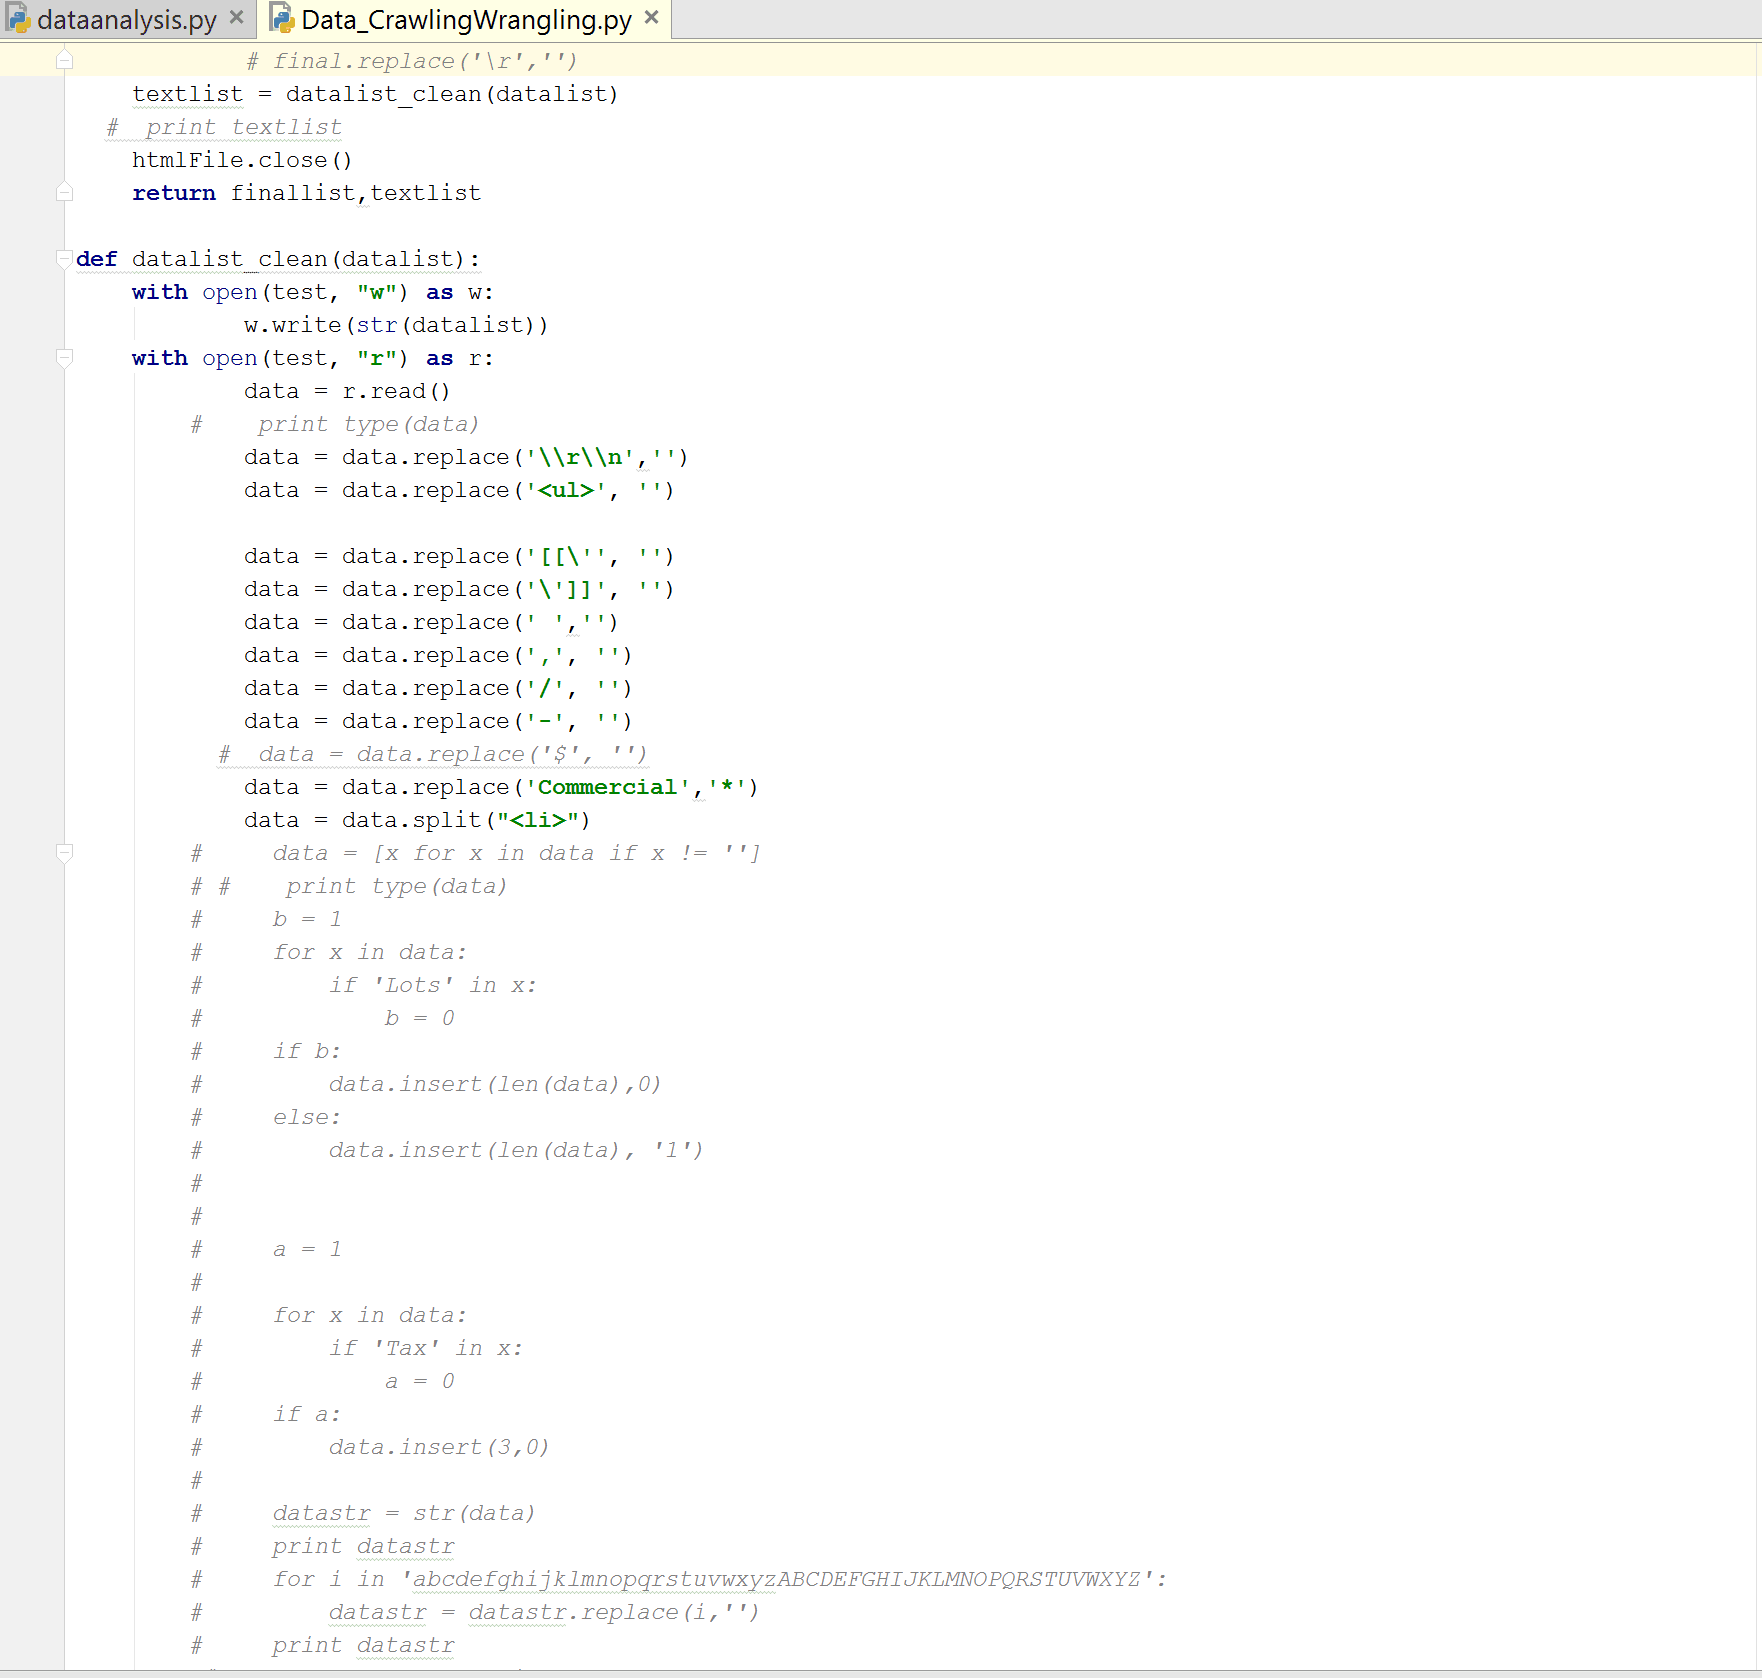
\includegraphics[width=0.5\textwidth]{datacrawling2.png}
\caption{}
\end{figure}
\begin{figure}
\centering
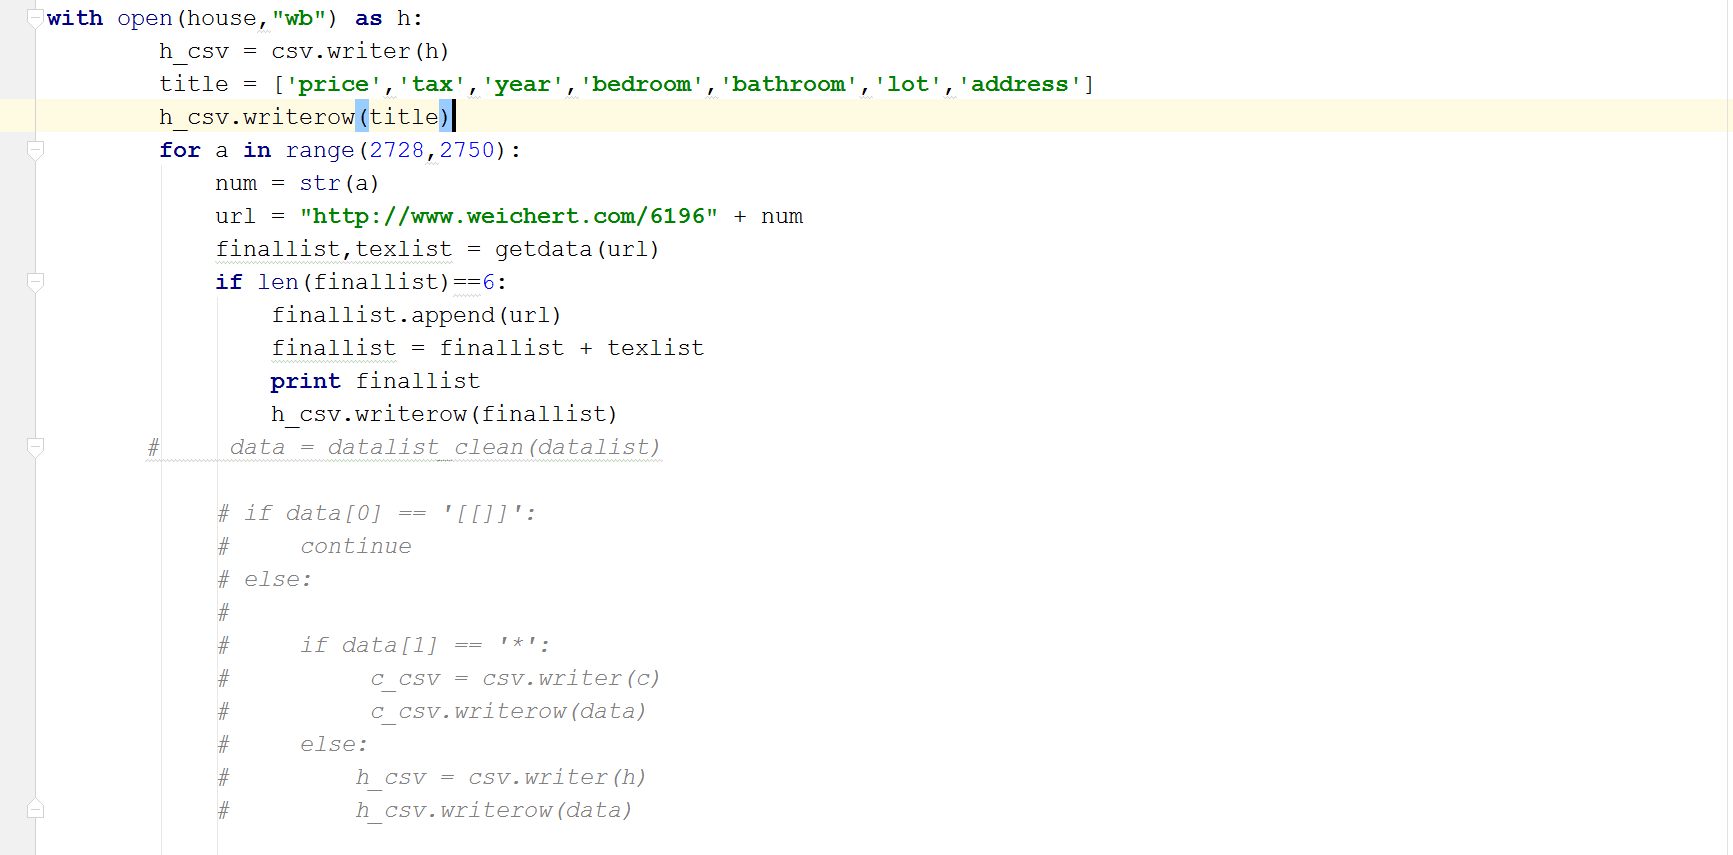
\includegraphics[width=0.5\textwidth]{datacrawling4.png}
\caption{}
\end{figure}
\item{DataAnalysis: See Fig.7-8}
\begin{figure}
\centering
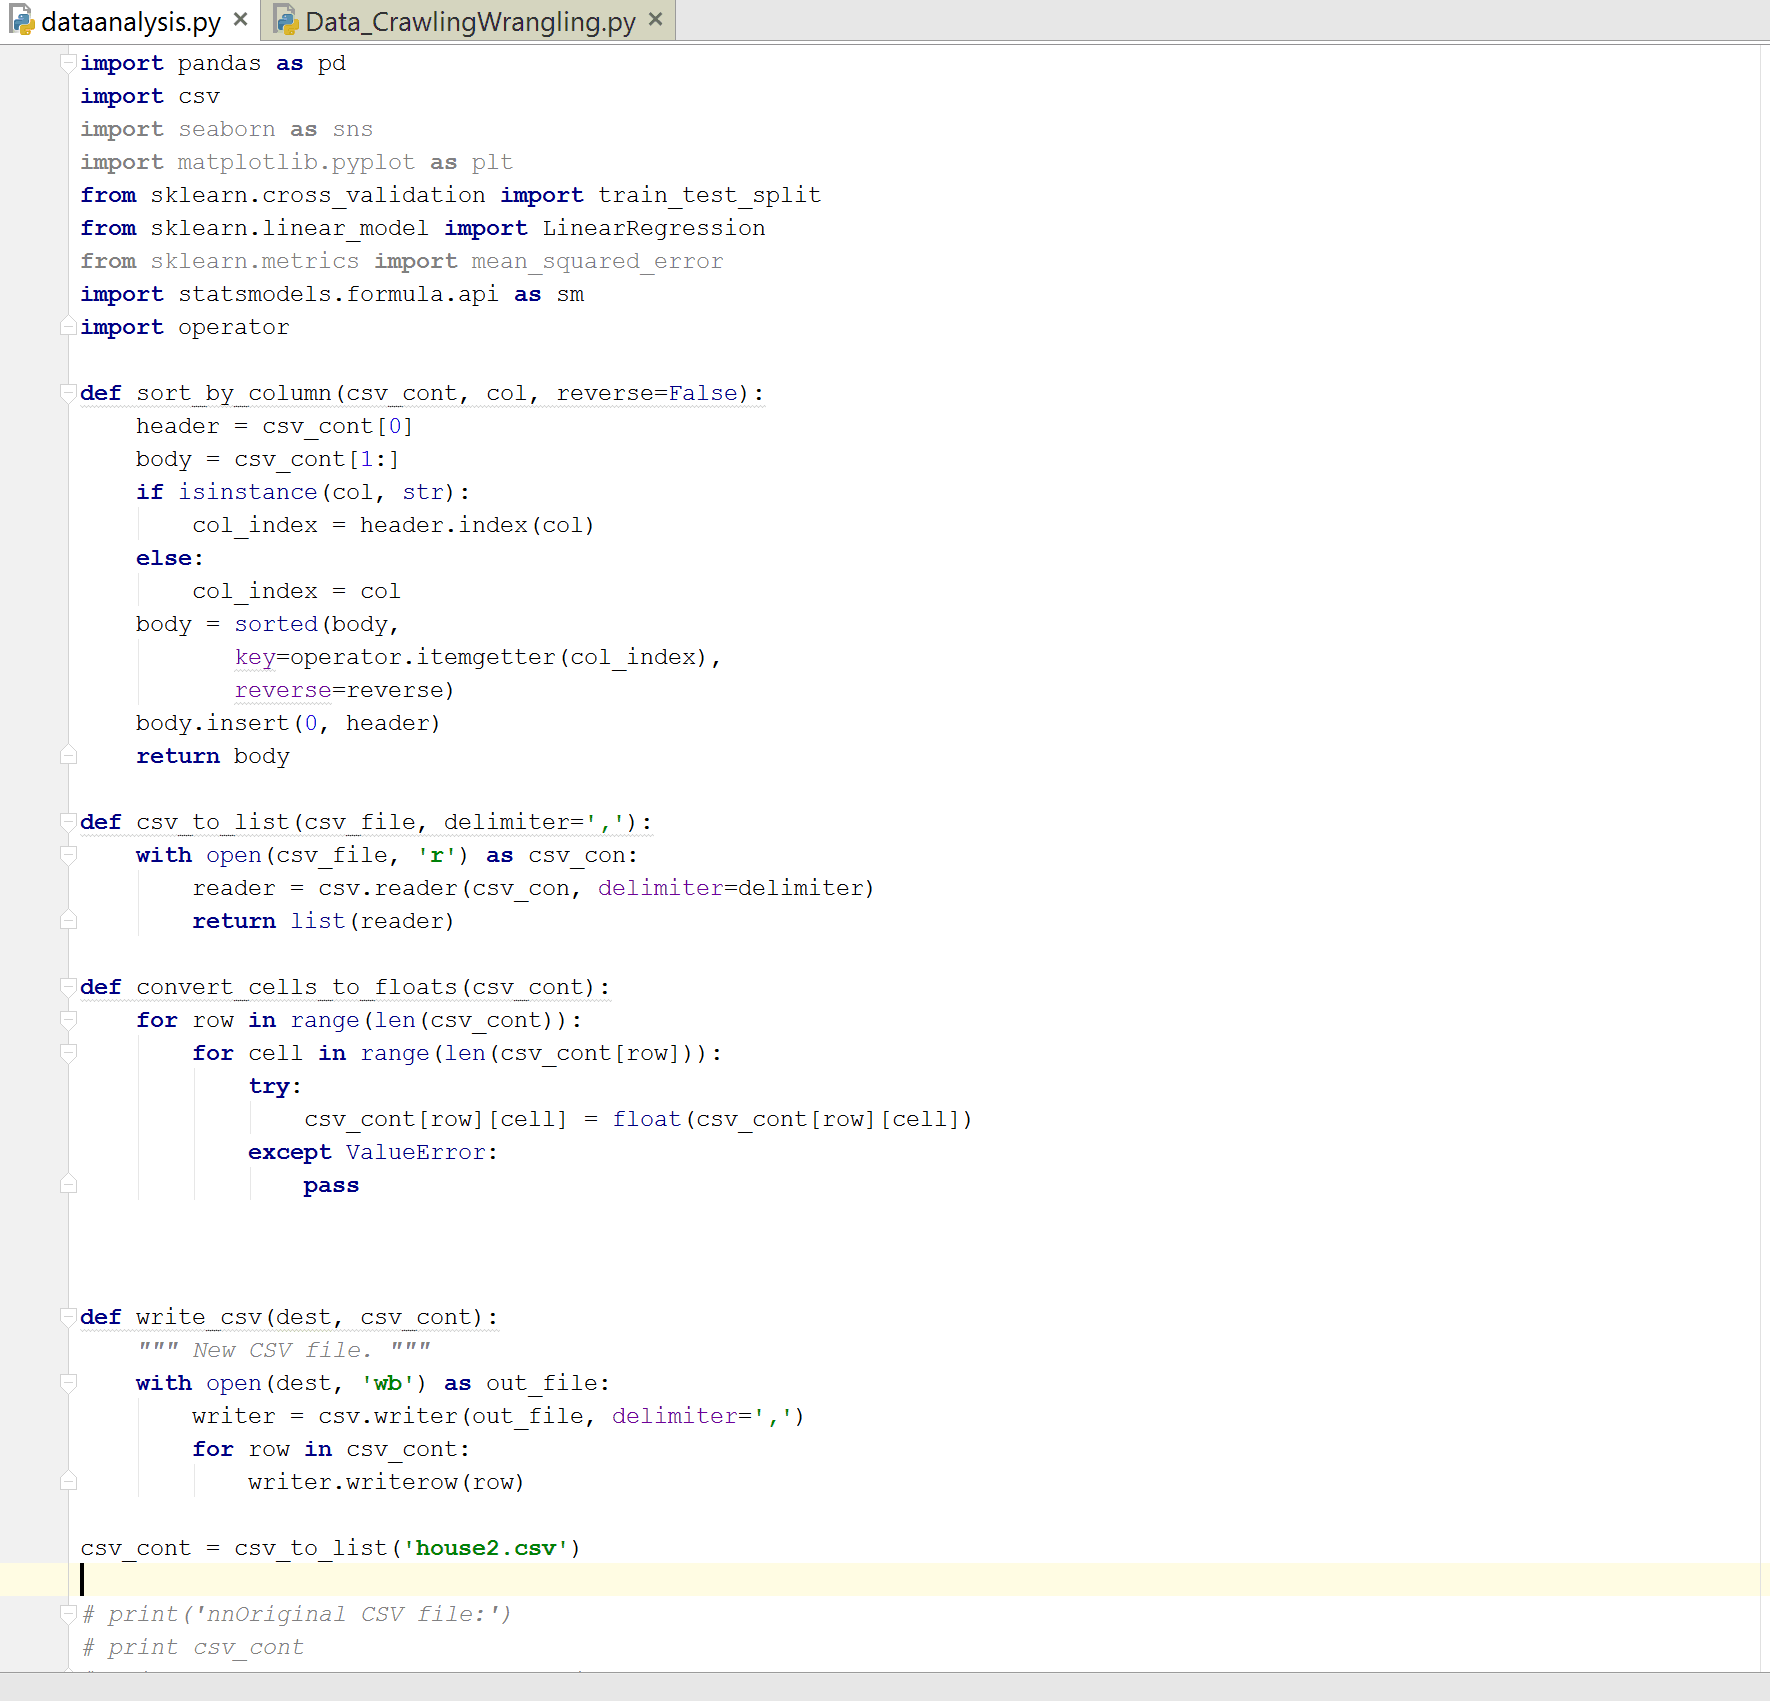
\includegraphics[width=0.5\textwidth]{DataAnalysis1.png}
\caption{}
\end{figure}
\begin{figure}
\centering
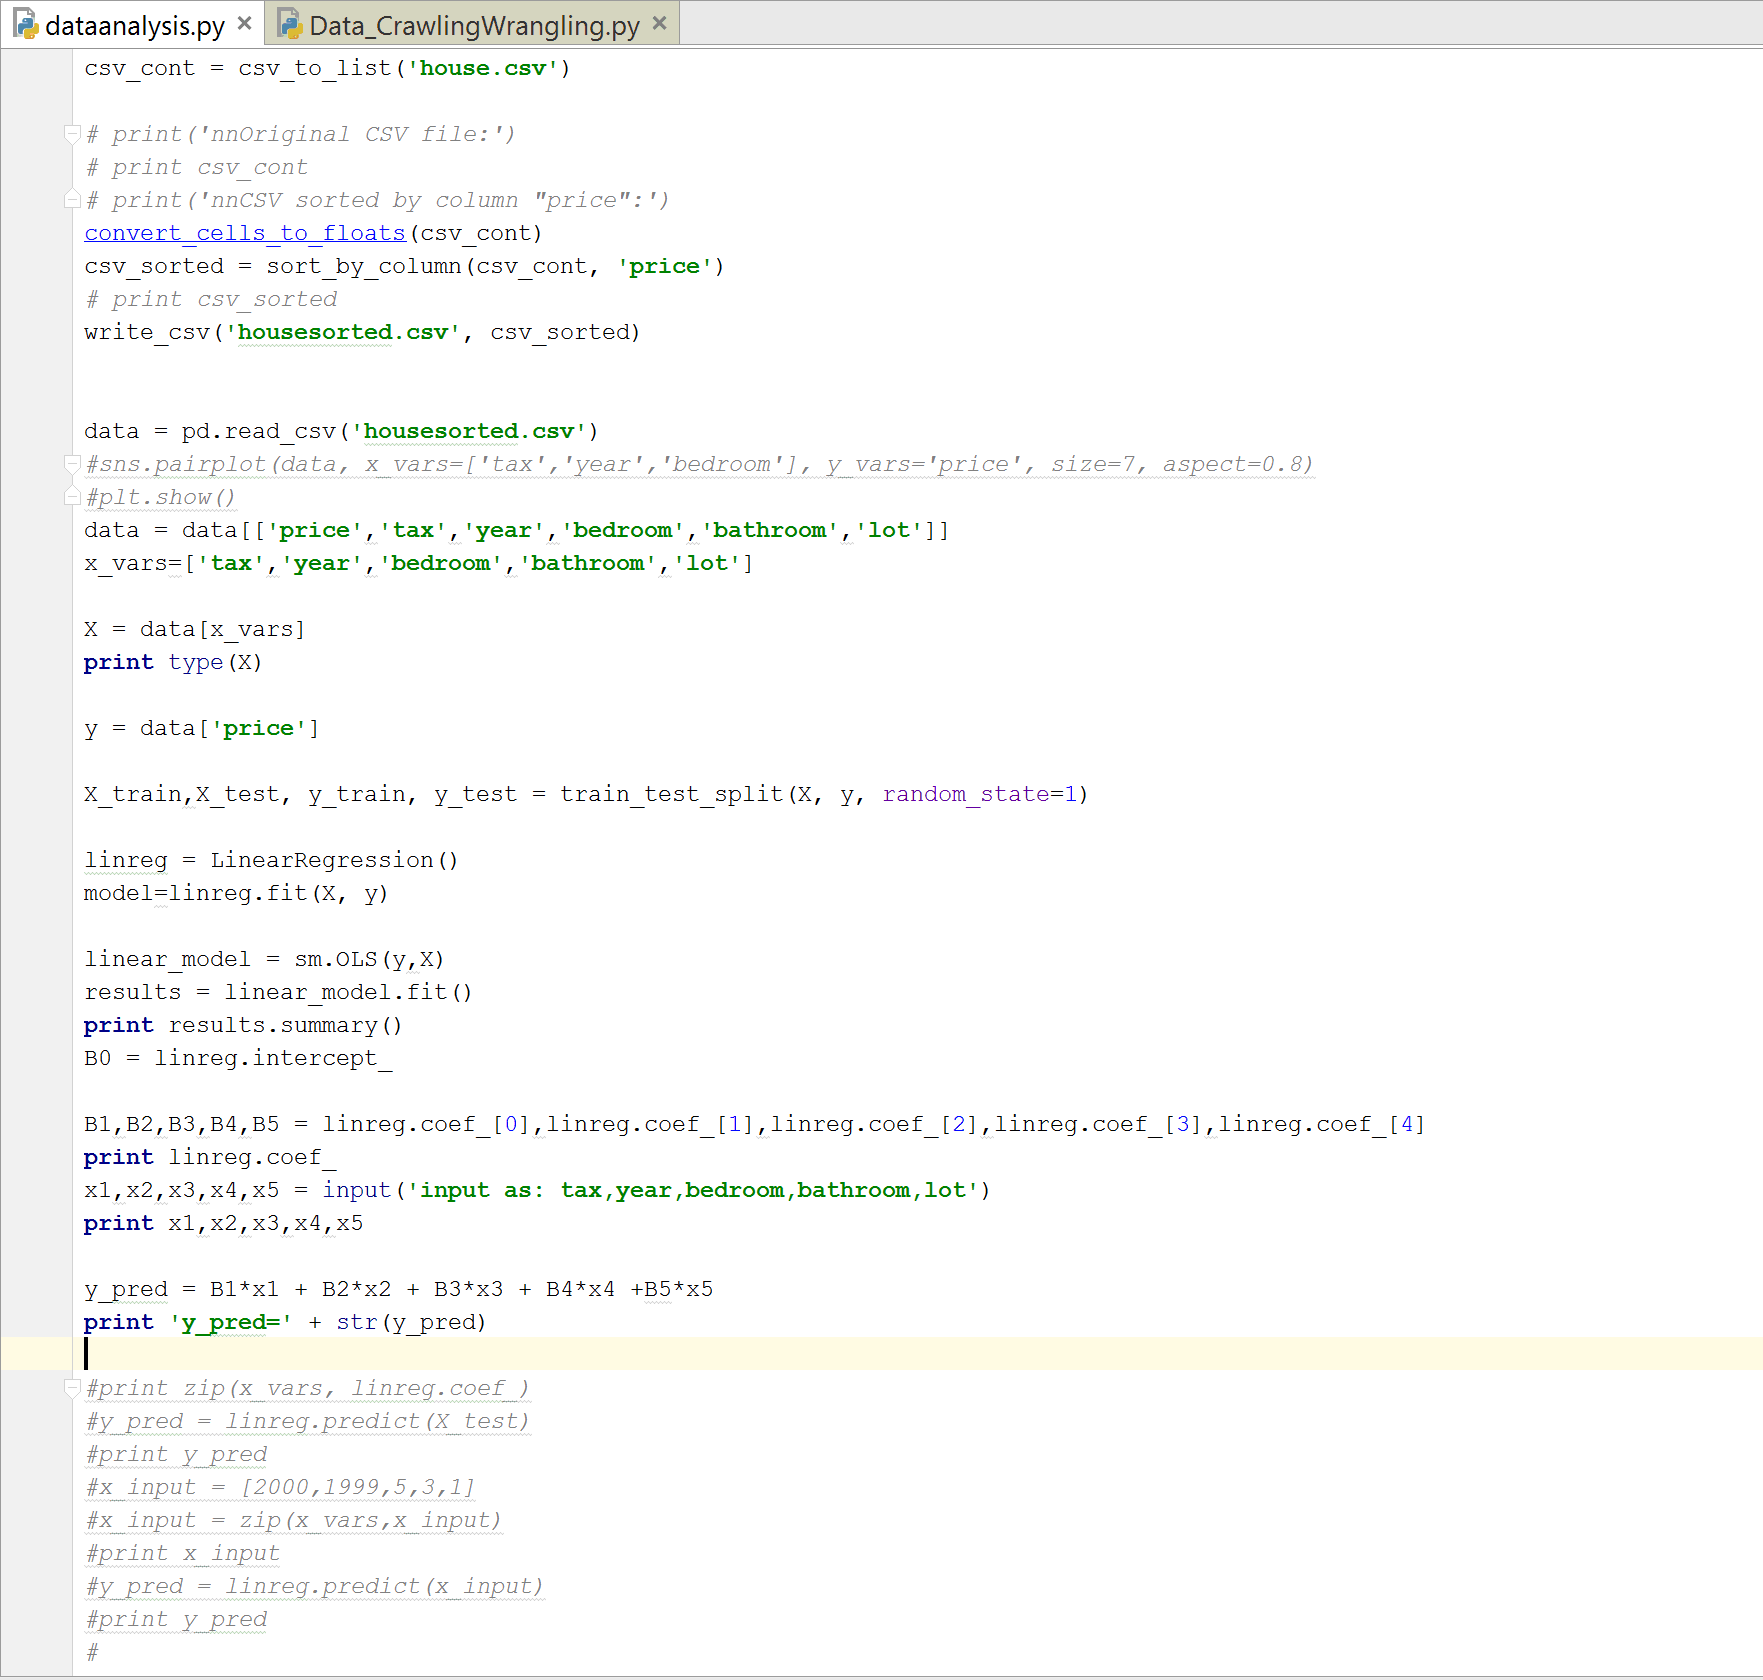
\includegraphics[width=0.5\textwidth]{DataAnalysis2.png}
\caption{}
\end{figure}
%The SQL table after the normalization steps (showing all table attributes).
\item{}
Demo and sample findings
%The SQL statements used to create the SQL tables, including the required triggers as well as the integrity constraints. At %least 2 triggers and 2 of each of the following constraint types have to exist in the project tables overall: 
\begin{itemize} 
\item{}
	Data size: 1MB;  Disk Resident: 10MB;  
\item{}
	 We collect houses' information from "weichert", calculate the prediction price through multiple linear regression.
	 After collecting all the information from the website, we find out that the built-year of houses have no effects on houses' prices. And this is weird, because in common sense, the elder the house is, the lower the price will be, considering higher cost on maintenance, lower security standard. Maybe the website does not put the built-year into the calculation standard.
%Whether some users will be denied access and/or updates to some data according to their roles (for example: student1 %can not access other students' ' grades, so a violation error pops up upon that action. Another example: a sales person %can see an item price, but can not change it, since only a manger can, also a violation error pops up upon that update %attempt).
\end{itemize}
\end{itemize}
}
